%%%%%%%%%%%%%%%%%%%%%%%%%%%%%%%%%%%%%%%%%
%  My documentation report
%  Objective: Explain what I did and how, in order to help someone continue with the investigation
%
% Important note:
% Chapter heading images should have a 2:1 width:height ratio,
% e.g. 920px width and 460px height.
%
% The images can be found anywhere, usually on sky surveys websites or the
% Astronomy Picture of the day archive http://apod.nasa.gov/apod/archivepix.html
%
% The original template (the Legrand Orange Book Template) can be found here --> http://www.latextemplates.com/template/the-legrand-orange-book
%
% Original author of the Legrand Orange Book Template:
% Mathias Legrand (legrand.mathias@gmail.com) with modifications by:
% Vel (vel@latextemplates.com)
%
% Original License:
% CC BY-NC-SA 3.0 (http://creativecommons.org/licenses/by-nc-sa/3.0/)
%%%%%%%%%%%%%%%%%%%%%%%%%%%%%%%%%%%%%%%%%
 
%----------------------------------------------------------------------------------------
%	PACKAGES AND OTHER DOCUMENT CONFIGURATIONS
%----------------------------------------------------------------------------------------

\documentclass[11pt,fleqn]{book} % Default font size and left-justified equations

\usepackage[top=3cm,bottom=3cm,left=3.2cm,right=3.2cm,headsep=10pt,letterpaper]{geometry} % Page margins

\usepackage{xcolor} % Required for specifying colors by name
\definecolor{ocre}{RGB}{52,177,201} % Define the orange color used for highlighting throughout the book

% Font Settings
\usepackage{avant} % Use the Avantgarde font for headings
%\usepackage{times} % Use the Times font for headings
\usepackage{mathptmx} % Use the Adobe Times Roman as the default text font together with math symbols from the Sym­bol, Chancery and Com­puter Modern fonts

\usepackage{microtype} % Slightly tweak font spacing for aesthetics
\usepackage[utf8]{inputenc} % Required for including letters with accents
\usepackage[T1]{fontenc} % Use 8-bit encoding that has 256 glyphs
\usepackage{array}
% Bibliography
\usepackage[style=alphabetic,sorting=nyt,sortcites=true,autopunct=true,babel=hyphen,hyperref=true,abbreviate=false,backref=true,backend=biber]{biblatex}
\addbibresource{bibliography.bib} % BibTeX bibliography file
\defbibheading{bibempty}{}

%%%%%%%%%%%%%%%%%%%%%%%%%%%%%%%%%%%%%%%%%
% This is based on the Legrand Orange Book
% Structural Definitions File
%
% The original template (the Legrand Orange Book Template) can be found here --> http://www.latextemplates.com/template/the-legrand-orange-book
%
% Original author of the Legrand Orange Book Template::
% Mathias Legrand (legrand.mathias@gmail.com) with modifications by:
% Vel (vel@latextemplates.com)
%
% Original License:
% CC BY-NC-SA 3.0 (http://creativecommons.org/licenses/by-nc-sa/3.0/)
%
%%%%%%%%%%%%%%%%%%%%%%%%%%%%%%%%%%%%%%%%%
%----------------------------------------------------------------------------------------
%	VARIOUS REQUIRED PACKAGES
%----------------------------------------------------------------------------------------

\usepackage{titlesec} % Allows customization of titles

\usepackage{graphicx} % Required for including pictures
\graphicspath{{Pictures/}} % Specifies the directory where pictures are stored

\usepackage{lipsum} % Inserts dummy text

\usepackage{tikz} % Required for drawing custom shapes

\usepackage[english]{babel} % English language/hyphenation

\usepackage{enumitem} % Customize lists
\setlist{nolistsep} % Reduce spacing between bullet points and numbered lists

\usepackage{booktabs} % Required for nicer horizontal rules in tables

\usepackage{eso-pic} % Required for specifying an image background in the title page

%----------------------------------------------------------------------------------------
%	MAIN TABLE OF CONTENTS
%----------------------------------------------------------------------------------------

\usepackage{titletoc} % Required for manipulating the table of contents

\contentsmargin{0cm} % Removes the default margin
% Chapter text styling
\titlecontents{chapter}[1.25cm] % Indentation
{\addvspace{15pt}\large\sffamily\bfseries} % Spacing and font options for chapters
{\color{ocre!60}\contentslabel[\Large\thecontentslabel]{1.25cm}\color{ocre}} % Chapter number
{}  
{\color{ocre!60}\normalsize\sffamily\bfseries\;\titlerule*[.5pc]{.}\;\thecontentspage} % Page number
% Section text styling
\titlecontents{section}[1.25cm] % Indentation
{\addvspace{5pt}\sffamily\bfseries} % Spacing and font options for sections
{\contentslabel[\thecontentslabel]{1.25cm}} % Section number
{}
{\sffamily\hfill\color{black}\thecontentspage} % Page number
[]
% Subsection text styling
\titlecontents{subsection}[1.25cm] % Indentation
{\addvspace{1pt}\sffamily\small} % Spacing and font options for subsections
{\contentslabel[\thecontentslabel]{1.25cm}} % Subsection number
{}
{\sffamily\;\titlerule*[.5pc]{.}\;\thecontentspage} % Page number
[] 

%----------------------------------------------------------------------------------------
%	MINI TABLE OF CONTENTS IN CHAPTER HEADS
%----------------------------------------------------------------------------------------

% Section text styling
\titlecontents{lsection}[0em] % Indendating
{\footnotesize\sffamily} % Font settings
{}
{}
{}

% Subsection text styling
\titlecontents{lsubsection}[.5em] % Indentation
{\normalfont\footnotesize\sffamily} % Font settings
{}
{}
{}
 
%----------------------------------------------------------------------------------------
%	PAGE HEADERS
%----------------------------------------------------------------------------------------

\usepackage{fancyhdr} % Required for header and footer configuration

\pagestyle{fancy}
\renewcommand{\chaptermark}[1]{\markboth{\sffamily\normalsize\bfseries\chaptername\ \thechapter.\ #1}{}} % Chapter text font settings
\renewcommand{\sectionmark}[1]{\markright{\sffamily\normalsize\thesection\hspace{5pt}#1}{}} % Section text font settings
\fancyhf{} \fancyhead[LE,RO]{\sffamily\normalsize\thepage} % Font setting for the page number in the header
\fancyhead[LO]{\rightmark} % Print the nearest section name on the left side of odd pages
\fancyhead[RE]{\leftmark} % Print the current chapter name on the right side of even pages
\renewcommand{\headrulewidth}{0.5pt} % Width of the rule under the header
\addtolength{\headheight}{2.5pt} % Increase the spacing around the header slightly
\renewcommand{\footrulewidth}{0pt} % Removes the rule in the footer
\fancypagestyle{plain}{\fancyhead{}\renewcommand{\headrulewidth}{0pt}} % Style for when a plain pagestyle is specified

% Removes the header from odd empty pages at the end of chapters
\makeatletter
\renewcommand{\cleardoublepage}{
\clearpage\ifodd\c@page\else
\hbox{}
\vspace*{\fill}
\thispagestyle{empty}
\newpage
\fi}

%----------------------------------------------------------------------------------------
%	THEOREM STYLES
%----------------------------------------------------------------------------------------

\usepackage{amsmath,amsfonts,amssymb,amsthm} % For math equations, theorems, symbols, etc

\newcommand{\intoo}[2]{\mathopen{]}#1\,;#2\mathclose{[}}
\newcommand{\ud}{\mathop{\mathrm{{}d}}\mathopen{}}
\newcommand{\intff}[2]{\mathopen{[}#1\,;#2\mathclose{]}}
\newtheorem{notation}{Notation}[chapter]

%%%%%%%%%%%%%%%%%%%%%%%%%%%%%%%%%%%%%%%%%%%%%%%%%%%%%%%%%%%%%%%%%%%%%%%%%%%
%%%%%%%%%%%%%%%%%%%% dedicated to boxed/framed environements %%%%%%%%%%%%%%
%%%%%%%%%%%%%%%%%%%%%%%%%%%%%%%%%%%%%%%%%%%%%%%%%%%%%%%%%%%%%%%%%%%%%%%%%%%
\newtheoremstyle{ocrenumbox}% % Theorem style name
{0pt}% Space above
{0pt}% Space below
{\normalfont}% % Body font
{}% Indent amount
{\small\bf\sffamily\color{ocre}}% % Theorem head font
{\;}% Punctuation after theorem head
{0.25em}% Space after theorem head
{\small\sffamily\color{ocre}\thmname{#1}\nobreakspace\thmnumber{\@ifnotempty{#1}{}\@upn{#2}}% Theorem text (e.g. Theorem 2.1)
\thmnote{\nobreakspace\the\thm@notefont\sffamily\bfseries\color{black}---\nobreakspace#3.}} % Optional theorem note
\renewcommand{\qedsymbol}{$\blacksquare$}% Optional qed square

\newtheoremstyle{blacknumex}% Theorem style name
{5pt}% Space above
{5pt}% Space below
{\normalfont}% Body font
{} % Indent amount
{\small\bf\sffamily}% Theorem head font
{\;}% Punctuation after theorem head
{0.25em}% Space after theorem head
{\small\sffamily{\tiny\ensuremath{\blacksquare}}\nobreakspace\thmname{#1}\nobreakspace\thmnumber{\@ifnotempty{#1}{}\@upn{#2}}% Theorem text (e.g. Theorem 2.1)
\thmnote{\nobreakspace\the\thm@notefont\sffamily\bfseries---\nobreakspace#3.}}% Optional theorem note

\newtheoremstyle{blacknumbox} % Theorem style name
{0pt}% Space above
{0pt}% Space below
{\normalfont}% Body font
{}% Indent amount
{\small\bf\sffamily}% Theorem head font
{\;}% Punctuation after theorem head
{0.25em}% Space after theorem head
{\small\sffamily\thmname{#1}\nobreakspace\thmnumber{\@ifnotempty{#1}{}\@upn{#2}}% Theorem text (e.g. Theorem 2.1)
\thmnote{\nobreakspace\the\thm@notefont\sffamily\bfseries---\nobreakspace#3.}}% Optional theorem note

%%%%%%%%%%%%%%%%%%%%%%%%%%%%%%%%%%%%%%%%%%%%%%%%%%%%%%%%%%%%%%%%%%%%%%%%%%%
%%%%%%%%%%%%% dedicated to non-boxed/non-framed environements %%%%%%%%%%%%%
%%%%%%%%%%%%%%%%%%%%%%%%%%%%%%%%%%%%%%%%%%%%%%%%%%%%%%%%%%%%%%%%%%%%%%%%%%%
\newtheoremstyle{ocrenum}% % Theorem style name
{5pt}% Space above
{5pt}% Space below
{\normalfont}% % Body font
{}% Indent amount
{\small\bf\sffamily\color{ocre}}% % Theorem head font
{\;}% Punctuation after theorem head
{0.25em}% Space after theorem head
{\small\sffamily\color{ocre}\thmname{#1}\nobreakspace\thmnumber{\@ifnotempty{#1}{}\@upn{#2}}% Theorem text (e.g. Theorem 2.1)
\thmnote{\nobreakspace\the\thm@notefont\sffamily\bfseries\color{black}---\nobreakspace#3.}} % Optional theorem note
\renewcommand{\qedsymbol}{$\blacksquare$}% Optional qed square
\makeatother

% Defines the theorem text style for each type of theorem to one of the three styles above
\newcounter{dummy} 
\numberwithin{dummy}{section}
\theoremstyle{ocrenumbox}
\newtheorem{theoremeT}[dummy]{Theorem}
\newtheorem{problem}{Problem}[chapter]
\newtheorem{exerciseT}{Exercise}[chapter]
\theoremstyle{blacknumex}
\newtheorem{exampleT}{Example}[chapter]
\theoremstyle{blacknumbox}
\newtheorem{vocabulary}{Vocabulary}[chapter]
\newtheorem{definitionT}{Definition}[section]
\newtheorem{corollaryT}[dummy]{Corollary}
\theoremstyle{ocrenum}
\newtheorem{proposition}[dummy]{Proposition}

%----------------------------------------------------------------------------------------
%	DEFINITION OF COLORED BOXES
%----------------------------------------------------------------------------------------

\RequirePackage[framemethod=default]{mdframed} % Required for creating the theorem, definition, exercise and corollary boxes

% Theorem box
\newmdenv[skipabove=7pt,
skipbelow=7pt,
backgroundcolor=black!5,
linecolor=ocre,
innerleftmargin=5pt,
innerrightmargin=5pt,
innertopmargin=5pt,
leftmargin=0cm,
rightmargin=0cm,
innerbottommargin=5pt]{tBox}

% Exercise box	  
\newmdenv[skipabove=7pt,
skipbelow=7pt,
rightline=false,
leftline=true,
topline=false,
bottomline=false,
backgroundcolor=ocre!10,
linecolor=ocre,
innerleftmargin=5pt,
innerrightmargin=5pt,
innertopmargin=5pt,
innerbottommargin=5pt,
leftmargin=0cm,
rightmargin=0cm,
linewidth=4pt]{eBox}	

% Definition box
\newmdenv[skipabove=7pt,
skipbelow=7pt,
rightline=false,
leftline=true,
topline=false,
bottomline=false,
linecolor=ocre,
innerleftmargin=5pt,
innerrightmargin=5pt,
innertopmargin=0pt,
leftmargin=0cm,
rightmargin=0cm,
linewidth=4pt,
innerbottommargin=0pt]{dBox}	

% Corollary box
\newmdenv[skipabove=7pt,
skipbelow=7pt,
rightline=false,
leftline=true,
topline=false,
bottomline=false,
linecolor=gray,
backgroundcolor=black!5,
innerleftmargin=5pt,
innerrightmargin=5pt,
innertopmargin=5pt,
leftmargin=0cm,
rightmargin=0cm,
linewidth=4pt,
innerbottommargin=5pt]{cBox}

% Creates an environment for each type of theorem and assigns it a theorem text style from the "Theorem Styles" section above and a colored box from above
\newenvironment{theorem}{\begin{tBox}\begin{theoremeT}}{\end{theoremeT}\end{tBox}}
\newenvironment{exercise}{\begin{eBox}\begin{exerciseT}}{\hfill{\color{ocre}\tiny\ensuremath{\blacksquare}}\end{exerciseT}\end{eBox}}				  
\newenvironment{definition}{\begin{dBox}\begin{definitionT}}{\end{definitionT}\end{dBox}}	
\newenvironment{example}{\begin{exampleT}}{\hfill{\tiny\ensuremath{\blacksquare}}\end{exampleT}}		
\newenvironment{corollary}{\begin{cBox}\begin{corollaryT}}{\end{corollaryT}\end{cBox}}	

%----------------------------------------------------------------------------------------
%	REMARK ENVIRONMENT
%----------------------------------------------------------------------------------------

\newenvironment{remark}{\par\vspace{10pt}\small % Vertical white space above the remark and smaller font size
\begin{list}{}{
\leftmargin=35pt % Indentation on the left
\rightmargin=25pt}\item\ignorespaces % Indentation on the right
\makebox[-2.5pt]{\begin{tikzpicture}[overlay]
\node[draw=ocre!60,line width=1pt,circle,fill=ocre!25,font=\sffamily\bfseries,inner sep=2pt,outer sep=0pt] at (-15pt,0pt){\textcolor{ocre}{R}};\end{tikzpicture}} % Orange R in a circle
\advance\baselineskip -1pt}{\end{list}\vskip5pt} % Tighter line spacing and white space after remark

%----------------------------------------------------------------------------------------
%	SECTION NUMBERING IN THE MARGIN
%----------------------------------------------------------------------------------------

\makeatletter
\renewcommand{\@seccntformat}[1]{\llap{\textcolor{ocre}{\csname the#1\endcsname}\hspace{1em}}}                    
\renewcommand{\section}{\@startsection{section}{1}{\z@}
{-4ex \@plus -1ex \@minus -.4ex}
{1ex \@plus.2ex }
{\normalfont\large\sffamily\bfseries}}
\renewcommand{\subsection}{\@startsection {subsection}{2}{\z@}
{-3ex \@plus -0.1ex \@minus -.4ex}
{0.5ex \@plus.2ex }
{\normalfont\sffamily\bfseries}}
\renewcommand{\subsubsection}{\@startsection {subsubsection}{3}{\z@}
{-2ex \@plus -0.1ex \@minus -.2ex}
{.2ex \@plus.2ex }
{\normalfont\small\sffamily\bfseries}}                        
\renewcommand\paragraph{\@startsection{paragraph}{4}{\z@}
{-2ex \@plus-.2ex \@minus .2ex}
{.1ex}
{\normalfont\small\sffamily\bfseries}}

%----------------------------------------------------------------------------------------
%	HYPERLINKS IN THE DOCUMENTS
%----------------------------------------------------------------------------------------

% For an unclear reason, the package should be loaded now and not later
\usepackage{hyperref}
\hypersetup{hidelinks,backref=true,pagebackref=true,hyperindex=true,colorlinks=false,breaklinks=true,urlcolor= ocre,bookmarks=true,bookmarksopen=false,pdftitle={Title},pdfauthor={Author}}

%----------------------------------------------------------------------------------------
%	CHAPTER HEADINGS
%----------------------------------------------------------------------------------------

% The set-up below should be (sadly) manually adapted to the overall margin page septup controlled by the geometry package loaded in the main.tex document. It is possible to implement below the dimensions used in the goemetry package (top,bottom,left,right)... TO BE DONE

\newcommand{\thechapterimage}{}
\newcommand{\chapterimage}[1]{\renewcommand{\thechapterimage}{#1}}

% Numbered chapters with mini tableofcontents
\def\thechapter{\arabic{chapter}}
\def\@makechapterhead#1{
\thispagestyle{empty}
{\centering \normalfont\sffamily
\ifnum \c@secnumdepth >\m@ne
\if@mainmatter
\startcontents
\begin{tikzpicture}[remember picture,overlay]
\node at (current page.north west)
{\begin{tikzpicture}[remember picture,overlay]
\node[anchor=north west,inner sep=0pt] at (0,0) {\includegraphics[width=\paperwidth]{\thechapterimage}};
%%%%%%%%%%%%%%%%%%%%%%%%%%%%%%%%%%%%%%%%%%%%%%%%%%%%%%%%%%%%%%%%%%%%%%%%%%%%%%%%%%%%%
% Commenting the 3 lines below removes the small contents box in the chapter heading
%\fill[color=ocre!10!white,opacity=.6] (1cm,0) rectangle (8cm,-7cm);
%\node[anchor=north west] at (1.1cm,.35cm) {\parbox[t][8cm][t]{6.5cm}{\huge\bfseries\flushleft \printcontents{l}{1}{\setcounter{tocdepth}{2}}}};
\draw[anchor=west] (5cm,-9cm) node [rounded corners=20pt,fill=ocre!10!white,text opacity=1,draw=ocre,draw opacity=1,line width=1.5pt,fill opacity=.6,inner sep=12pt]{\huge\sffamily\bfseries\textcolor{black}{\thechapter. #1\strut\makebox[22cm]{}}};
%%%%%%%%%%%%%%%%%%%%%%%%%%%%%%%%%%%%%%%%%%%%%%%%%%%%%%%%%%%%%%%%%%%%%%%%%%%%%%%%%%%%%
\end{tikzpicture}};
\end{tikzpicture}}
\par\vspace*{230\p@}
\fi
\fi}

% Unnumbered chapters without mini tableofcontents (could be added though) 
\def\@makeschapterhead#1{
\thispagestyle{empty}
{\centering \normalfont\sffamily
\ifnum \c@secnumdepth >\m@ne
\if@mainmatter
\begin{tikzpicture}[remember picture,overlay]
\node at (current page.north west)
{\begin{tikzpicture}[remember picture,overlay]
\node[anchor=north west,inner sep=0pt] at (0,0) {\includegraphics[width=\paperwidth]{\thechapterimage}};
\draw[anchor=west] (5cm,-9cm) node [rounded corners=20pt,fill=ocre!10!white,fill opacity=.6,inner sep=12pt,text opacity=1,draw=ocre,draw opacity=1,line width=1.5pt]{\huge\sffamily\bfseries\textcolor{black}{#1\strut\makebox[22cm]{}}};
\end{tikzpicture}};
\end{tikzpicture}}
\par\vspace*{230\p@}
\fi
\fi
}
\makeatother % Insert the commands.tex file which contains the majority of the structure behind the template
\newcolumntype{L}[1]{>{\raggedright\let\newline\\\arraybackslash\hspace{0pt}}m{#1}}
\newcolumntype{C}[1]{>{\centering\let\newline\\\arraybackslash\hspace{0pt}}m{#1}}
\newcolumntype{R}[1]{>{\raggedleft\let\newline\\\arraybackslash\hspace{0pt}}m{#1}}
\begin{document}
\title{Basics Makes You Smarter}

%----------------------------------------------------------------------------------------
%	TITLE PAGE
%----------------------------------------------------------------------------------------

\begingroup
\thispagestyle{empty}
\AddToShipoutPicture*{\put(0,0){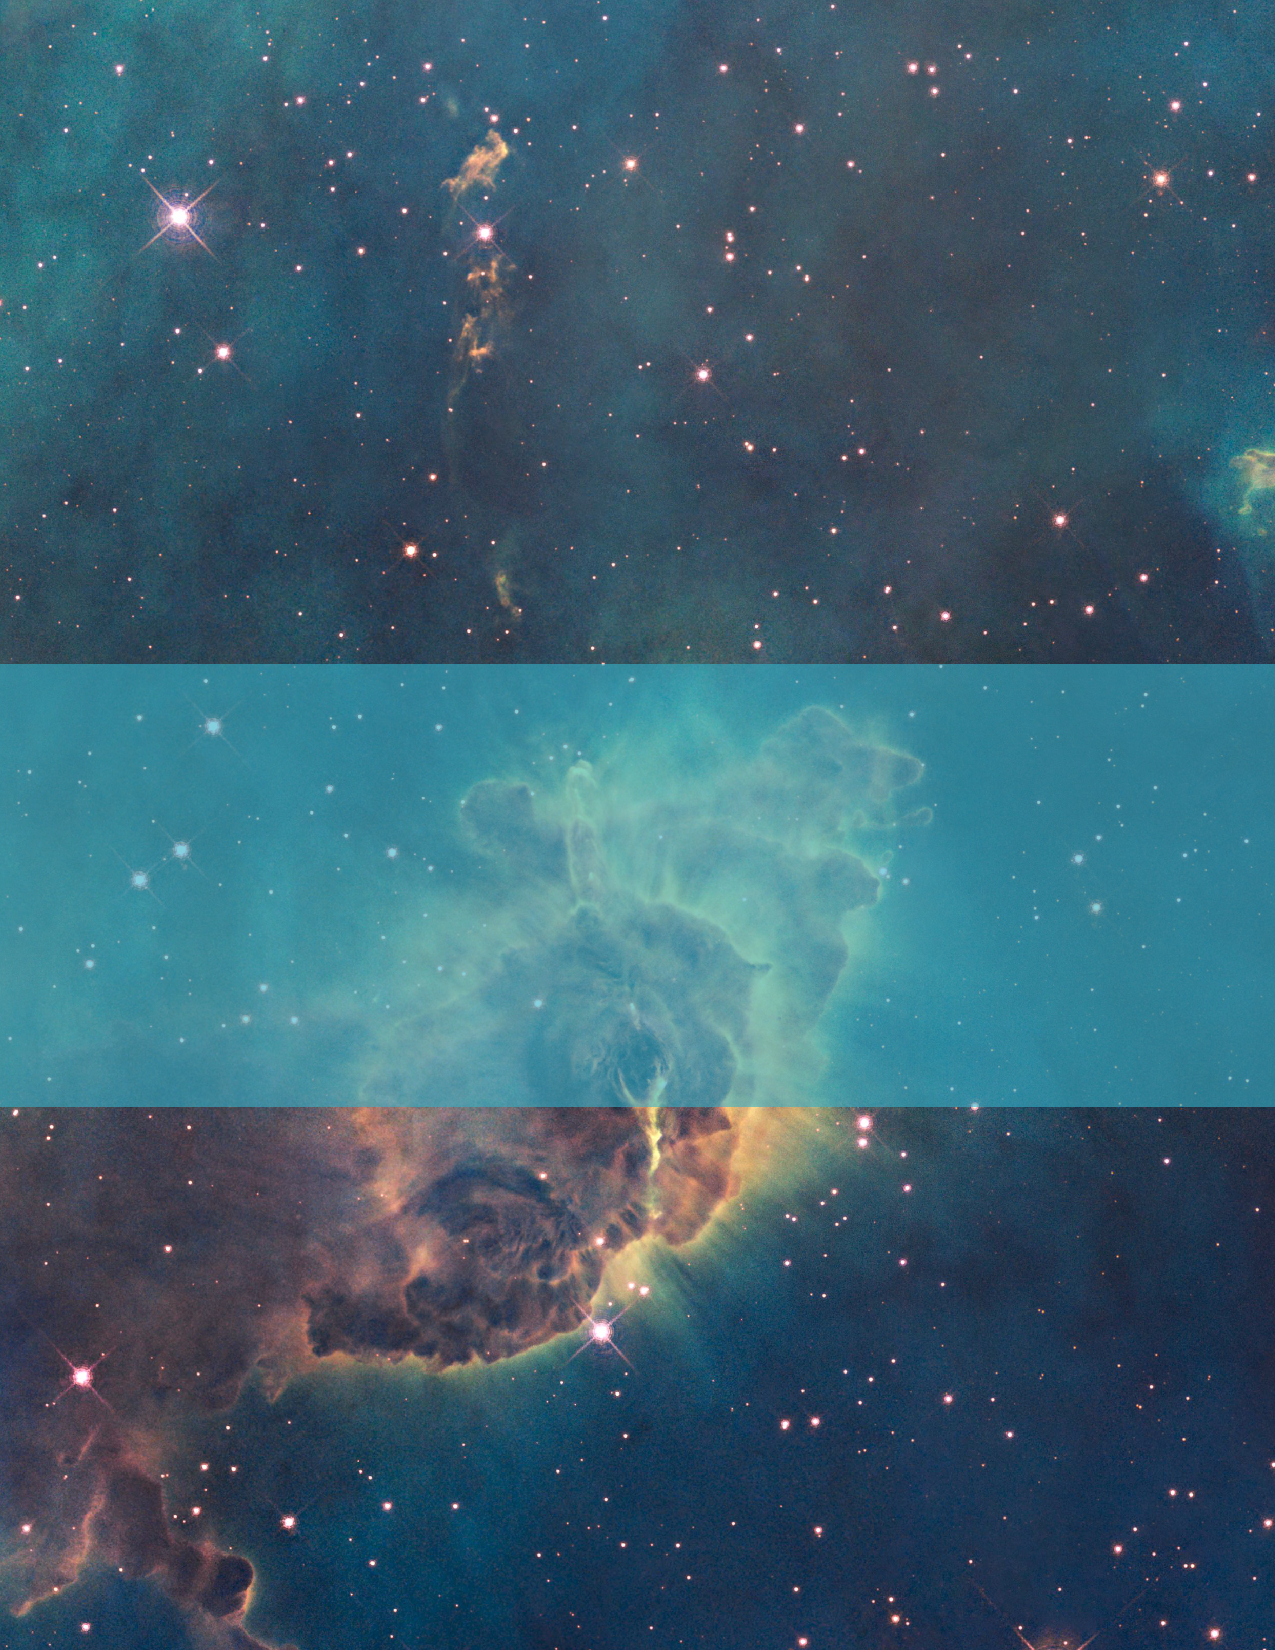
\includegraphics[scale=1.25]{esahubble}}} % Image background
\centering
\vspace*{5cm}
\par\normalfont\fontsize{35}{35}\sffamily\selectfont
\textbf{Basics Makes You Smarter}\\
{\LARGE Making The Way to Physics Easier}\par % Book title
\vspace*{1cm}
{\Huge Asif Ikbal}\par % Author name
\endgroup

%----------------------------------------------------------------------------------------
%	COPYRIGHT PAGE
%----------------------------------------------------------------------------------------

\newpage
~\vfill
\thispagestyle{empty}

%\noindent Copyright \copyright\ 2014 Andrea Hidalgo\\ % Copyright notice

%\noindent \textsc{Summer Research Internship, University of Western Ontario}\\

%\noindent \textsc{github.com/LaurethTeX/Clustering}\\ % URL

%\noindent This research was done under the supervision of Dr. Pauline Barmby with the financial support of the MITACS Globalink Research Internship Award within a total of 12 weeks, from June 16th to September 5th of 2014.\\ % License information

%\noindent \textit{First release, August 2014} % Printing/edition date

%----------------------------------------------------------------------------------------
%	TABLE OF CONTENTS
%----------------------------------------------------------------------------------------

\chapterimage{head1.png} % Table of contents heading image

\pagestyle{empty} % No headers

\tableofcontents % Print the table of contents itself

%\cleardoublepage % Forces the first chapter to start on an odd page so it's on the right

\pagestyle{fancy} % Print headers again



\chapterimage{head2.png} % Chapter heading image

\chapter{Albegra}
\section{Basic Laws of Algebra}
The basic laws of algebra are the associative, commutative and distributive laws. They help explain the relationship between number operations and lend toward simplifying equations or solving them.
%https://en.wikiversity.org/wiki/Basic_Laws_of_Algebra
\begin{table}[h]
	\centering
	\begin{tabular}{|m{4cm}|c|m{6cm}|}
		\hline
		Property Name & Definition & Example \\ \hline
		Commutative Law for addition & $a+b = b+ a$ & $2+3 = 3+2 = 5$ \\ \hline
		Commutative law for multiplication & $a * b = b * a$ & $2 * 3 = 3 * 2 = 6$ \\ \hline
		Associative law for addition & $(a+b) + c = a + (b+c)$ & $(2+3) + 4 = 5 + 4 = 9$ and\newline $2 + (3+4) = 2 + 7 = 9$ \\ \hline
		Associative law for multiplication & $(a*b)*c = a* (b*c)$ & $(2*3) *4 = 6*4 = 24$ and\newline$2*(3*4) = 2*12=24$ \\ \hline
		Distributive law & $a*(b+c) = (a*b) + (a*c)$ & $2(3+4) = 2*7=14$ and\newline  $2(3+4) = 2*3 + 2*4 = 6+8 = 14$ \\
		\hline
	\end{tabular}
	\caption{Basic Laws of Algebra}
\end{table}
\newpage
\section{Pythagorean Theorem}

In mathematics, the Pythagorean theorem, also known as Pythagoras' theorem, is a fundamental relation in Euclidean geometry among the three sides of a right triangle. It states that the square of the hypotenuse (the side opposite the right angle) is equal to the sum of the squares of the other two sides. The theorem can be written as an equation relating the lengths of the sides a, b and c, often called the "Pythagorean equation.

\begin{equation}
a^2 + b^2 = c^2
\end{equation}
If the length of both a and b are known, then c can be calculated as	
%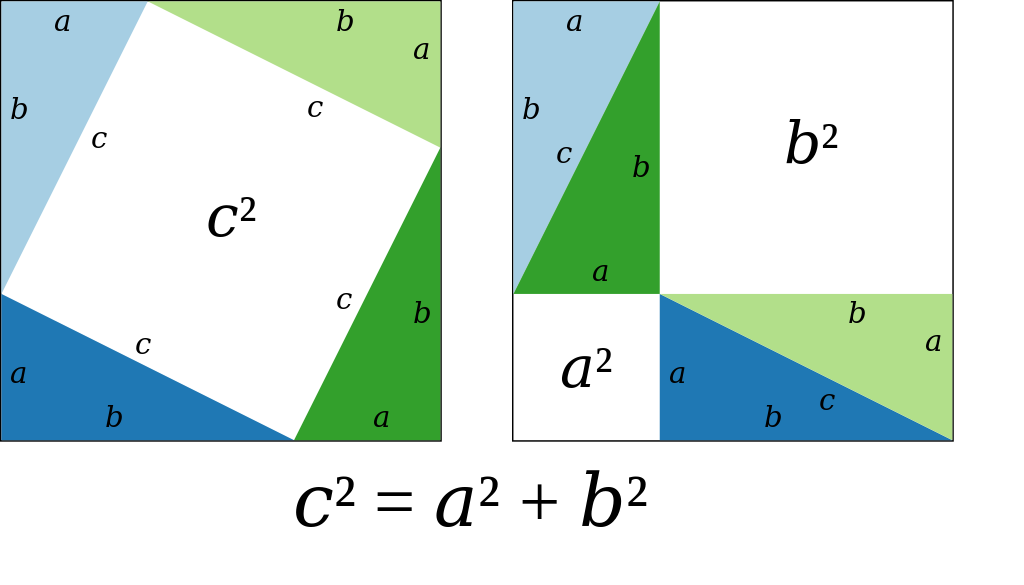
\includegraphics[width=55mm,left]{01}
\begin{equation}
c = \sqrt{a^2+b^2}
\end{equation}
If the length of the hypotenuse c and of one side (a or b) are known, then the length of the other side can be calculated as

\begin{equation}
a = \sqrt{c^2-b^2}
\end{equation}
or
\begin{equation}
b = \sqrt{c^2-a^2}
\end{equation}
The Pythagorean equation relates the sides of a right triangle in a simple way, so that if the lengths of any two sides are known the length of the third side can be found. Another corollary of the theorem is that in any right triangle, the hypotenuse is greater than any one of the other sides, but less than their sum.

\section{Logarithm}
	The logarithm to base 10 (that is b = 10) is called the common logarithm and has many applications in science and engineering. The natural logarithm has the number e (that is$b  \approx 2.718$) as its base; its use is widespread in mathematics and physics, because of its simpler derivative. The binary logarithm uses base 2 (that is b = 2) and is commonly used in computer science.
	
	
	\begin{align*}
		10^0 &= 1 \\
		10^1 &= 10 \\
		10^2 &= 100 \\
		10^3 &= 1000 \\
	\end{align*}
	
	
	\begin{equation}
	\log_{10}(100) = 2
	\end{equation}
	\begin{equation}
	\log_{10}(10^2) = 2
	\end{equation}
	\begin{equation}
	10^{\log_{10}(100)} = 100
	\end{equation}
	\begin{equation}
	\log_{b} (a) = \log_{b} (b^c)= c
	\end{equation}
	\begin{equation}
	b^{\log b^a} = b^c = b^{\log b^{(b^c)}} = a
	\end{equation}
	\begin{equation}
	\log^{(ab)} = \log a +\log b
	\end{equation}
	
	Example: 1
	\begin{displaymath}
	If \quad y = \log e^x
	\end{displaymath}
	\begin{displaymath}
	=> e^y=e^{(10ye^x)} = x
	\end{displaymath}
	\begin{displaymath}
	=> \frac{de^x}{dx} = \frac{dx}{dx} = 1
	\end{displaymath}
	\begin{displaymath}
	=>\frac{de^y}{dx} \frac{dy}{dx} = 1
	\end{displaymath}
	\begin{displaymath}
	=>e^y \frac{dy}{dx} = 1
	\end{displaymath}
	\begin{displaymath}
	=>e^{-y}e^y\frac{dy}{dx} = e^{-y}
	\end{displaymath}
	\begin{displaymath}
	=>e^{-y+y}\frac{dy}{dx} = e^{-y}
	\end{displaymath}
	\begin{displaymath}
	=>e^0\frac{dy}{dx} = e^{-y}
	\end{displaymath}
	\begin{displaymath}
	=>\frac{dy}{dx} = e^{-y}
	\end{displaymath}
	\begin{displaymath}
	=> \frac{d\ln x}{dx} = e^{-\ln x}
	\end{displaymath}
	\begin{displaymath}
	=> e^{\ln\big(\frac{1}{x}\big)}
	\end{displaymath}
	\begin{displaymath}
	=> \frac{1}{x}
	\end{displaymath}
	\newline
	Example: 2
	\begin{equation}
	x^h ;\quad \frac{dx^h}{dx} = hx^{h-1}
	\end{equation}
	\begin{equation}
	a^x; \quad \frac{da^x}{dx} = a^x\ln a;\frac{de^x}{dx} = e^x
	\end{equation}
	\begin{equation}
	log x; \frac{d\log x}{dx} = \frac{1}{x}\bigg(\bigg)
	\end{equation}
	\begin{equation}
	\frac{d\ln x}{dx} = \frac{1}{x}
	\end{equation}
	\newline
	\begin{equation}
	\log\bigg(\frac{a}{b}\bigg) = \log a - \log b
	\end{equation}
	\begin{equation}
	\log(ab)=\log a + \log b
	\end{equation}
	\begin{equation}
	\log \bigg(\frac{1}{b}\bigg) = \log 1-\log b
	\end{equation}
	\begin{displaymath}
	=> 0 - \log b
	\end{displaymath}
	\begin{displaymath}
	=> - \log b
	\end{displaymath}
	\newline
	Example: 3
	\begin{displaymath}
	f(x) = a^x
	\end{displaymath}
	\begin{displaymath}
	=> y = a^x
	\end{displaymath}
	\begin{displaymath}
	=> \ln y=\ln a^x
	\end{displaymath}
	\begin{displaymath}
	=> \frac{d\ln y}{dy} = \frac{d(x\ln a)}{dx}
	\end{displaymath}
	\begin{displaymath}
	=>\frac{d\ln y}{dy}\frac{dy}{dx} = \bigg(\frac{dy}{dx}\bigg)\ln a
	\end{displaymath}
	\begin{displaymath}
	=> \frac{1}{y}\frac{dy}{dx} = \ln a
	\end{displaymath}
	\begin{displaymath}
	=> \frac{dy}{dx} = y\ln a
	\end{displaymath}
	\begin{displaymath}
	=>\frac{da^x}{dx} = a^x\ln a 
	\end{displaymath}
	\newline
	\begin{equation}
	\frac{d\ln x}{dx} = \frac{1}{x} ....................................
	\end{equation}
	\newline
	(Base 10)
	\newline
	Example: 10
	\begin{displaymath}
	f(x) = \log10^x
	\end{displaymath}
	\begin{displaymath}
	y = \log x
	\end{displaymath}
	\begin{displaymath}
	=> 10^y = 10^{\log x} = x
	\end{displaymath}
	\begin{displaymath}
	=>\frac{d10^y}{dx} = \frac{dx}{dx} = 1
	\end{displaymath}
	\begin{displaymath}
	=> \frac{d10^y}{dy}\frac{dy}{dx} = 1
	\end{displaymath}
	\begin{displaymath}
	=> 10^y \ln (10) \frac{dy}{dx} = 1
	\end{displaymath}
	\begin{displaymath}
	=>x \ln (10)\frac{dy}{dx} = 1
	\end{displaymath}
	\begin{displaymath}
	=> \frac{dy}{dx} = \frac{d\log}{dx} = \frac{1}{x\ln(10)}
	\end{displaymath}
	\newline
	***
	
	***
	

%This statement requires citation \cite{book_key}; this one is more specific \cite[122]{article_key}.

\graphicspath{ {./Pictures/} }
%----------------------------------------------------------------------------------------
%	CHAPTER 2
%----------------------------------------------------------------------------------------
\chapterimage{band1.png}


\chapter{Trigonometry}

\subsection{Introduction}
Trigonometry is most simply associated with planar right-angle triangles (each of which is a two-dimensional triangle with one angle equal to 90 degrees). The applicability to non-right-angle triangles exists, but, since any non-right-angle triangle (on a flat plane) can be bisected to create two right-angle triangles, most problems can be reduced to calculations on right-angle triangles. Thus the majority of applications relate to right-angle triangles.
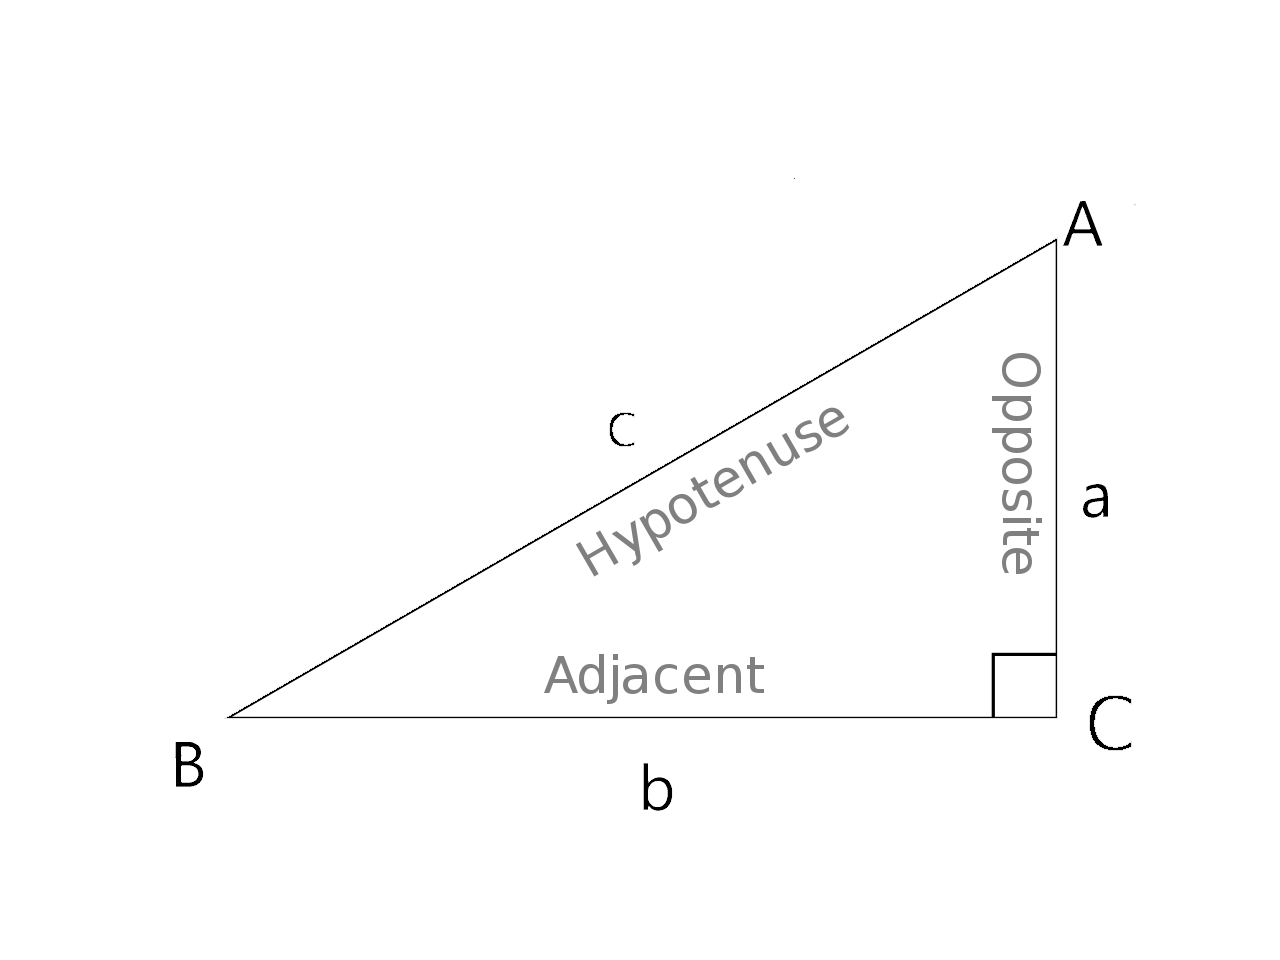
\includegraphics[width=50mm]{3}
One exception to this is spherical trigonometry, the study of triangles on spheres, surfaces of constant positive curvature, in elliptic geometry (a fundamental part of astronomy and navigation). Trigonometry on surfaces of negative curvature is part of hyperbolic geometry.
\newline
Define:
\newline
\begin{equation}
\sin\theta = \frac{Opposite}{Hypotenuse} = \frac{b}{c}
\end{equation}
\begin{equation}
\cos\theta = \frac{Adjacent}{Hypotenuse} = \frac{a}{c}
\end{equation}
\begin{equation}
\tan\theta = \frac{\sin\theta}{\cos\theta}= \frac{b/c}{a/c} = \frac{Opposite}{Adjacent} = \frac{b}{a}
\end{equation}
\newpage
Example: 1
\begin{equation}
a^2+b^2=c^2
\end{equation}
\begin{displaymath}
=>\frac{a^2}{c^2}+\frac{b^2}{c^2} = 1
\end{displaymath}
\begin{displaymath}
=> \bigg(\frac{a}{c}\bigg)^2 + \bigg(\frac{b}{c}\bigg)^2 = 1
\end{displaymath}
\begin{displaymath}
=> (\cos\theta)^2+(\sin\theta)^2 = 1
\end{displaymath}
\begin{equation}
\cos^2\theta+\sin^2\theta = 1
\end{equation}
\newline
\begin{equation}
Cotangent->\cot\theta = \frac{1}{\tan\theta} = \frac{a}{b} = \frac{\cos\theta}{\sin\theta}
\end{equation}
\begin{equation}
Secant->\sec\theta = \frac{1}{\cos\theta} = \frac{c}{a}
\end{equation}
\begin{equation}
Cosecant->\cosh\theta = \frac{1}{\sin\theta}=\frac{c}{b}
\end{equation}
\newline
Example: 2
\begin{equation}
a^2+b^2=c^2
\end{equation}
\begin{displaymath}
=>1+\frac{b^2}{c^2}=\bigg(\frac{c}{a}\bigg)^2
\end{displaymath}
\begin{displaymath}
=> 1+\bigg(\frac{b}{a}\bigg)^2=\bigg(\frac{c}{a}\bigg)^2
\end{displaymath}
\begin{displaymath}
=> 1+\tan^2\theta = \sec^2\theta
\end{displaymath}
\newline
Example: 3
\begin{equation}
a^2+b^2=c^2
\end{equation}
\begin{displaymath}
=>\frac{a^2}{b^2}+1 = \frac{c^2}{b^2}
\end{displaymath}
\begin{displaymath}
=> \bigg(\frac{a}{b}\bigg)^2+1= \bigg(\frac{c}{b}\bigg)^2
\end{displaymath}
\begin{displaymath}
=> \cot^2\theta+1=\cosh^2\theta
\end{displaymath}







\graphicspath{ {./Pictures/} }
%----------------------------------------------------------------------------------------
%	CHAPTER 3
%----------------------------------------------------------------------------------------

\chapterimage{boat.png}
\chapter{Calculus}
\section{Differentiation}

	In mathematics, differential calculus is a subfield of calculus concerned with the study of the rates at which quantities change.
	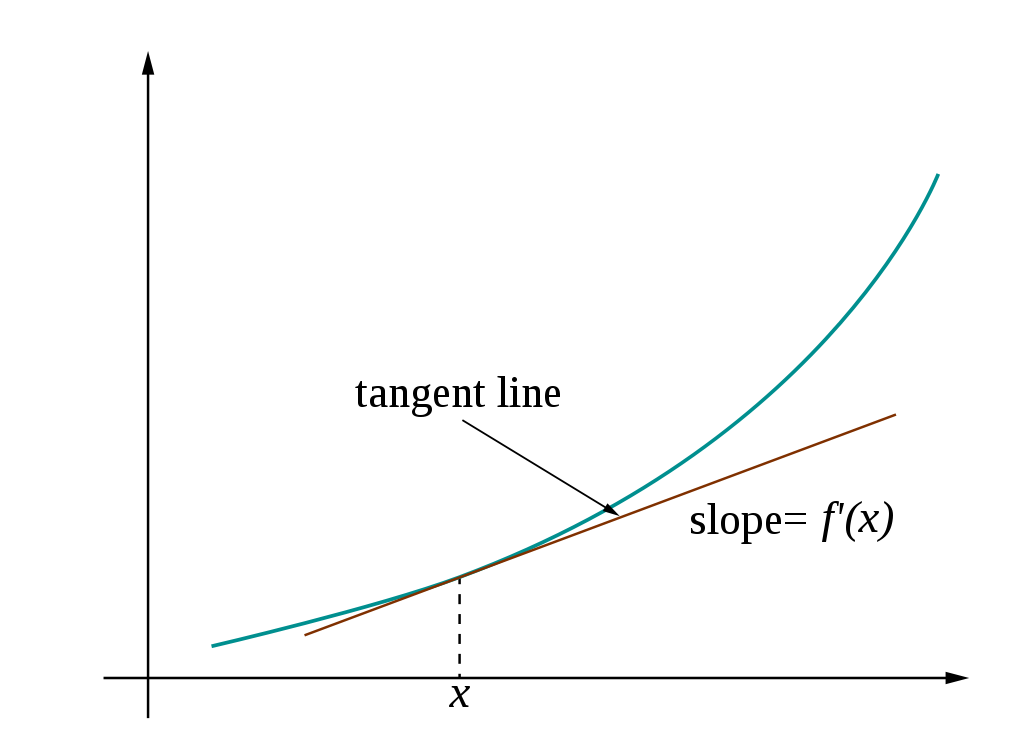
\includegraphics[width=50mm]{02}
	It is one of the two traditional divisions of calculus, the other being integral calculus, the study of the area beneath a curve.
	
	\begin{equation}
	\frac{duv}{dx}=\frac{du}{dx}v+u\frac{du}{dx}
	\end{equation}
	\begin{displaymath}
	\frac{df(x)}{dx} = \frac{f(x+h)-f(x)}{h}
	\end{displaymath}
	\begin{displaymath}
	=> \frac{(f+df)-(f)}{dx}
	\end{displaymath}
	\begin{displaymath}
	=>\frac{df}{dx}
	\end{displaymath}
	\newline
	\begin{displaymath}
	\frac{duv}{dx} = \frac{(u+du)(v+du)-uv}{dx}
	\end{displaymath}
	\begin{displaymath}
	=>\frac{(uv+du+udv+dudv)-uv}{dx}
	\end{displaymath}
	\begin{displaymath}
	=> \frac{duv+duv+dudv}{dx}
	\end{displaymath}
	\begin{displaymath}
	=> \frac{duv+udv}{dx}
	\end{displaymath}
	\begin{displaymath}
	=> \frac{du}{dx}v+u\frac{dv}{dx}
	\end{displaymath}
	\newline
	\begin{displaymath}
	\frac{df}{dx} = \frac{f_2-f_1}{x_2-x_1}
	\end{displaymath}
	\begin{displaymath}
	=>\frac{(f_1+df)-f_1}{x_2-x_1}
	\end{displaymath}
	\begin{displaymath}
	=>\frac{(f_1+df)-f_1}{dx}
	\end{displaymath}
	
	\subsection{Compound angle in trigonometry function}
	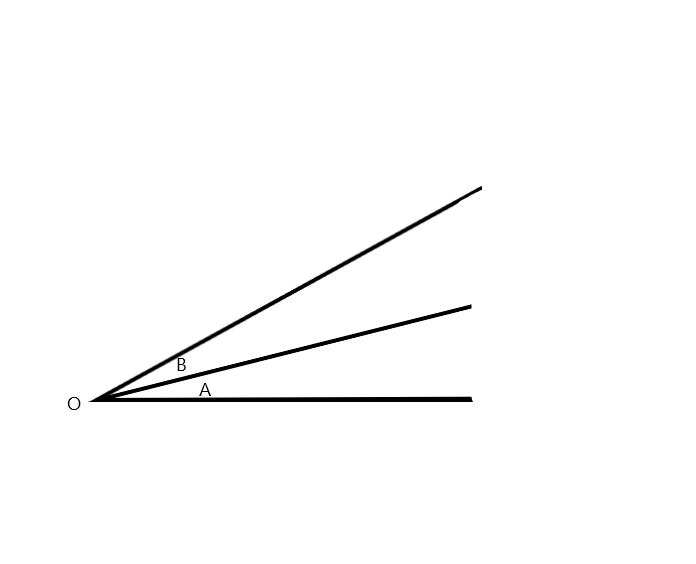
\includegraphics[width=60mm]{5}
	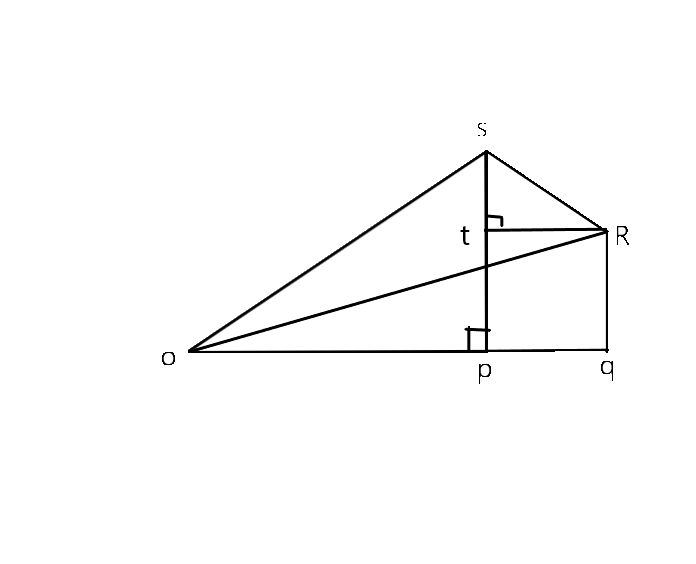
\includegraphics[width=60mm]{4}
	\newline
	Example
	\begin{equation}
	\sin(A+B)=\frac{sp}{os}
	\end{equation}
	\begin{displaymath}
	=>\frac{st+tp}{os}
	\end{displaymath}
	\begin{displaymath}
	=>\frac{st}{os}+\frac{tp}{os}
	\end{displaymath}
	\begin{displaymath}
	=>\frac{st}{sr}\frac{sr}{os}+\frac{tp}{os}
	\end{displaymath}
	\begin{displaymath}
	=>\frac{st}{sr}\frac{sr}{os}+\frac{ra}{or}\frac{or}{os}
	\end{displaymath}
	\begin{displaymath}
	=> \cos A\sin B+\sin A\cos B
	\end{displaymath}
	\begin{equation}
	\sin(A+B) = \sin A\cos B+\cos A\sin B
	\end{equation}
	
	\includegraphics[width=60mm]{8}
	\newline
	Example:
	\newline
	\begin{displaymath}
	\cos(\alpha+\beta) = \frac{EA}{AD}
	\end{displaymath}
	\begin{displaymath}
	=> \frac{GA}{AD}-\frac{FH}{AD}
	\end{displaymath}
	\begin{displaymath}
	=> \frac{GA}{AF}\frac{AF}{AD}-\frac{FH}{DF}
	\end{displaymath}
	\begin{displaymath}
	=> \frac{GA}{AF}\frac{AF}{AD}-\frac{FH}{DF}\frac{DF}{AD}
	\end{displaymath}
	\begin{equation}
	=> \cos\alpha \cos\beta + \sin\alpha \sin\beta
	\end{equation}
	
	\subsection{Differentiation of trigonometric functions}
	\begin{equation}
	\sin(A+B) = \sin A\cos B+\cos A\sin B
	\end{equation}
	\begin{equation}
	\cos(A+B) = \cos A\cos B - \sin A\sin B
	\end{equation}
	\begin{equation}
	\frac{df(x)}{dx} = \frac{f(x+h)-x}{h}
	\end{equation}
	\newline
	Example: 1
	\begin{displaymath}
	\frac{d\sin(x)}{dx} = \frac{\sin x \cos h+\cos x\sin h-\sin x}{h}
	\end{displaymath}
	\begin{displaymath}
	=> \frac{\sin x + h\cos x - \sin x}{h}
	\end{displaymath}
	\begin{displaymath}
	=>\frac{h\cos x}{h}
	\end{displaymath}
	\begin{equation}
	\frac{d\sin(x)}{dx} = \cos x
	\end{equation}
	\newline
	Example: 2
	\begin{displaymath}
	\frac{d\cos(x)}{dx} = \frac{\cos(c+h)-\cos (x)}{h}
	\end{displaymath}
	\begin{displaymath}
	=> \frac{\cos x \cos h-\sin x \sin h - \cos x}{h}
	\end{displaymath}
	\begin{displaymath}
	=> \frac{cos x- h \cos x - \cos x}{h}
	\end{displaymath}
	\begin{displaymath}
	=> \frac{-h\sin x}{h}
	\end{displaymath}
	\begin{equation}
	\frac{d\cos (X)}{dx} = -\sin x
	\end{equation}
	\newline
	Example: 3
	\begin{displaymath}
	\frac{d\tan x}{dx}
	\end{displaymath}
	\begin{displaymath}
	=>\frac{d}{dx}\bigg(\frac{\sin x}{cos x}\bigg)
	\end{displaymath}
	\begin{displaymath}
	=>\frac{d}{dx}(\sin x)\frac{1}{\cos x}+\sin x \frac{d}{dx}\bigg(\frac{1}{\cos x}\bigg)
	\end{displaymath}
	\begin{displaymath}
	=>\cos x \frac{1}{\cos x}+\sin x\frac{d}{dx}(\cos x)^{-1}
	\end{displaymath}
	\begin{displaymath}
	=> 1+\sin x\bigg[(-1)(\cos x)^{-2}\frac{d\cos x}{dx}\bigg]
	\end{displaymath}
	\begin{displaymath}
	=> 1+\sin x\frac{-1}{\cos x^2}(-\sin x)
	\end{displaymath}
	\begin{equation}
	\frac{d \tan x}{dx} = 1 + \tan^2 x
	\end{equation}

	\subsection{Properties of Differential Operator}
	\subsection{Chain Rule}
	
	\begin{displaymath}
	\frac{df(g(x))}{dx} = \frac{df(g(x))}{dg(x)}\frac{dy(x)}{dx}
	\end{displaymath}
	\begin{equation}
	\frac{df(g(x))}{dx} = \frac{df(x)}{dy}\frac{dg(x)}{dx}
	\end{equation}
	\newline
	Example: 1
	\begin{equation}
	Proof\,that\, \quad\frac{de^{x^2}}{dx} = 2x \, e^{x^2}
	\end{equation}
	\begin{displaymath}
	Let, \quad x^2 = y
	\end{displaymath}
	\begin{displaymath}
	=> \frac{de^2}{dx}
	\end{displaymath}
	\begin{displaymath}
	=> \frac{de^y}{dy}\frac{dy}{dx}
	\end{displaymath}
	\begin{displaymath}
	e^y\frac{dx^2}{dx}
	\end{displaymath}
	\begin{displaymath}
	e^y\,2x
	\end{displaymath}
	\begin{displaymath}
	=> 2x\,e^{x^2}
	\end{displaymath}	
	\newline
	Example: 2
	\begin{displaymath}
	\frac{d\sin(x^3)}{dx}
	\end{displaymath}	 
	\begin{displaymath}
	=> \frac{d \sin(x^3)}{dx}\frac{d(x^3)}{dx}
	\end{displaymath}
	\begin{displaymath}
	=> \cos(x^3) \,3x^2
	\end{displaymath}
	\newline
	\begin{equation}
	\frac{d(2x^2)}{dx} = \frac{2(x+h)^2-2x^2}{h} = 2\Big[\frac{(x+h)^2-x^2}{h}\Big] = 2\frac{dx^2}{dx}=2.2x=4x
	\end{equation}
	\begin{equation}
	\frac{d(cf(x))}{dx} = c\frac{df(x)}{dx}\quad (c)\,\,is\,\,a\,\,number 
	\end{equation}
	\begin{equation}
	\frac{d}{dx}\bigg(c_1f(x)+c_2f(x)\bigg)=\frac{d}{dx}\bigg((c_1+c_2)f(x)\bigg)
	\end{equation}
	\begin{equation}
	\frac{d}{dx}\bigg(c_1u(x)+c_2v(x)\bigg)=c_1\frac{du(x)}{dx}+c_2\frac{dv(x)}{dx}
	\end{equation}
	c, are number. f(x), u(x), v(x) are function
	\newline
	\begin{equation}
	\frac{d\sin(2x^3)}{dx} = \frac{d\sin(2x^3)}{d2x^3}\frac{dx^3}{dx} = \cos(2x^3)\frac{2(x+h)^3-22x^3}{h}=\cos(2x^3)2\frac{dx^3}{dx}=\cos(2x^3)2\,3x^3=\cos(2x^3)6x^3
	\end{equation}
	\begin{equation}
	\frac{de^{\sin(3x)}}{dx}=\frac{de^{\sin(3x)}}{d\sin(3x)}\frac{d\sin(3x)}{dx}=e^{\sin(3x)}\frac{d\sin(3x)}{d3x}\frac{d3x}{dx} = e^{\sin(3x)}\cos(3x)3x
	\end{equation}
	
	\subsection{Differentiation of Fundamental Functions}
	(1) Differentiation Property:
	\begin{equation}
	\frac{d(uv)}{dx} = \frac{du}{dx}v+u\frac{du}{dx}
	\end{equation}
	\begin{equation}
	\frac{d}{dx}(uv)=\frac{du}{dx}v+u\frac{du}{dx}
	\end{equation}
	\begin{equation}
	\frac{d}{dx}(f(x)g(x)=\frac{df(x)}{dx}\bigg(g(x)+f(x)\frac{dg(x)}{dx}\bigg)
	\end{equation}
	\newline
	(2) Scalar multiplication:
	\begin{equation}
	\frac{dcf(x)}{dx} = c\frac{df(x)}{dx}
	\end{equation}
	d, c is a number or constant
	\begin{equation}
	\frac{d}{dx}\Big((x+d)u(x)\Big)=c\frac{du}{dx}+d\frac{du}{dx}
	\end{equation}
	\begin{equation}
	\frac{d}{dx}\Big(c(u+v)\Big) = c\frac{du}{dx} + c\frac{dv}{dx}
	\end{equation}

\section{Integration}
\subsection{Fundamental Theorem of Calculus}

\begin{equation}
\int_{a}^{b}f(x)dx=F(b)-F(a)
\end{equation}
\begin{equation}
\frac{dF(x)}{dx}=f(x)
\end{equation}

Derivative of F(x) gives the slope of F(x) at a point integration of (x) the area under carve in the range of integration.Here it is [a, b]
\newline
\begin{equation}
f(x_1)h+f(x_2)h+f(x_3)h
\end{equation}
\begin{equation}
\int f(x)dx=f(x_1)dx+f(x_2)dx+......+f(x_n)dx
\end{equation}
Example: 1
\begin{equation}
\frac{dx^n}{dx} = nx^{n-1}
\end{equation}
\begin{equation}
\frac{dx^2}{dx} = 2x => F(x)=x^2
\end{equation}
\begin{displaymath}
f(x) = 2x
\end{displaymath}
\begin{displaymath}
\int_{0}^{2}f(x)dx=\int_{0}^{2}(2x)dx = F(5)-F(0)
\end{displaymath}
\begin{displaymath}
=> x^2\prod_{0}^{2}
\end{displaymath}
\begin{displaymath}
=>2^2-0^2
\end{displaymath}
\begin{displaymath}
=>4
\end{displaymath}
\newline
\begin{equation}
Area \,\, of \,\, triangle\,\, = \frac{1}{2}(base)(height)
\end{equation}
\begin{displaymath}
=>\frac{1}{2}*2*4
\end{displaymath}
\begin{displaymath}
=> 4
\end{displaymath}
Note: Area of triangle bh = 1/2 bh+ 1/2 bh
\newline
Example: 2
\begin{equation}
\int_{0}^{\frac{\pi}{2}}\cos xdx = \sin\big(\frac{\pi}{2}\big) - \sin(0)
\end{equation}
Example: 3
\begin{equation}
\int e^x dx = e^x+c
\end{equation}
Example: 4
\begin{equation}
\int f(x)dx=F(x)+c
\end{equation}
\begin{equation}
\int x^3 dx = \frac{1}{4}x^3+c	
\end{equation}
\begin{displaymath}
\frac{1}{4}\frac{dx^4}{dx} = x^3
\end{displaymath}

\section{Taylor Series}

One of the most importent thing in physics
\begin{equation}
f(x) = f(x_0)+(x-x_0)\frac{f^\prime(x_0)}{1!}+(x-x_0)^2\frac{f^{\prime\prime}(x_0)}{2!}+(x-x_0)^3\frac{f^{\prime\prime\prime}(x_0)}{3!}+.......
\end{equation}
\begin{equation}
f(x) = a_0+a_1x+a_2x^2+a_3x^3+a_4x^4+........
\end{equation}
In taylor series we expand/express a function as a polynomial.
\newline
\begin{equation}
= f(x_0)+\frac{x-x_0}{1!}\frac{df(x)}{dx}+\frac{(x-x_0)^2}{2!}\frac{d^2f(x)}{dx^2}+\frac{(x-x_0)^3}{3!}\frac{d^3f(x)}{dx^3}+....
\end{equation}
\begin{equation}
(1).... \quad \frac{df(x)}{dx} = f^\prime(x)
\end{equation}
\begin{equation}
(2).... \quad \frac{d}{dx}\bigg(\frac{df(x)}{dx}\bigg) = \frac{d^2f(x)}{dx^2} = f^{\prime\prime}(x)
\end{equation}
\begin{equation}
(3).... \quad \frac{d}{dx}\bigg(\frac{d}{dx}\bigg(\frac{df(x)}{dx}\bigg)\bigg) = \frac{d^3f(x)}{dx^3} = f^{\prime\prime\prime}(x)
\end{equation}
\newpage
Example: 1
\begin{displaymath}
f(x) = e^x
\end{displaymath}
Expanding around, $ x_0 = 0 $	
\begin{displaymath}
f(x_0) = f(0) = e^0=1
\end{displaymath}
\begin{displaymath}
f^\prime(x_0)=f^\prime(0)=e^0=1
\end{displaymath}
\begin{displaymath}
f^{\prime\prime}(x_0)=f^{\prime\prime}(0)=e^0=1
\end{displaymath}
\begin{displaymath}
f^{\prime\prime\prime}(x_0)=f^{\prime\prime\prime}(0)=e^0=1
\end{displaymath}
\begin{displaymath}
so \,\, f(x) = e^x=1+\frac{(x-x_0)}{1!}+\frac{(x-0)^2}{2!}+\frac{(x-0)^3}{3!}+......
\end{displaymath}
\begin{displaymath}
e^x = 1 + x+\frac{x^2}{2!}+\frac{x^3}{3!}+\frac{x^4}{4!}+.......
\end{displaymath}
\newline
Example: 2
\begin{displaymath}
f(x) = \sin x
\end{displaymath}
Expanding Around $ x_0 = 0 $
\begin{displaymath}
f(0) = \sin 0 = 0
\end{displaymath}
\begin{displaymath}
f^\prime(x)=\cos x =f^\prime(0)=\cos 0 = 1
\end{displaymath}
\begin{displaymath}
f^{\prime\prime}(x)=-\sin x = f^{\prime\prime}(0)= -\sin x = 0
\end{displaymath}
\begin{displaymath}
f^{\prime\prime\prime}(x)=-\cos x = f^{\prime\prime\prime}(0)=-\cos 0 = -1
\end{displaymath}
\begin{displaymath}
f(x)=f(0)+xf^\prime(x_0)+\frac{x^2}{2!}f^{\prime\prime}(x_0)+\frac{x_3}{3!}f^{\prime\prime\prime}(x_0)+....
\end{displaymath}
\begin{displaymath}
\sin x = 0+x+0+\frac{x^3}{3!}(-1)+.....
\end{displaymath}
\begin{displaymath}
\sin x = x-\frac{x^3}{3!}+\frac{x^5}{5!}-\frac{x^7}{7!}+......
\end{displaymath}
\newline
Example: 3
\begin{displaymath}
f(x)= \cos x
\end{displaymath}
Expanding around $ x_0=0 $
\begin{displaymath}
f(x) = \cos 0 = 1
\end{displaymath}
\begin{displaymath}
f^\prime(x) = -\sin x = f^\prime(0)=-\sin(0) = 0
\end{displaymath}
\begin{displaymath}
f^{\prime\prime}(x) = - \cos x = f^{\prime\prime}(0)= -\cos(0) = -1
\end{displaymath}
\begin{displaymath}
f^{\prime\prime\prime}(x)= \sin x = f^{\prime\prime\prime}(0)=\sin(0)= 0
\end{displaymath}
\begin{displaymath}
f^{\prime\prime\prime\prime}(x)= \cos x = f^{\prime\prime\prime\prime}(0)=\cos x = 1
\end{displaymath}
\begin{displaymath}
f(x) = f(0)+xf^\prime(x_0)+\frac{x^2}{2!}f^{\prime\prime}(x_0)+\frac{x^3}{3!}f^{\prime\prime\prime}(x_0)+\frac{x^4}{4!}
f^{\prime\prime\prime\prime}(x_0)+.......
\end{displaymath}
\begin{displaymath}
\cos x = 1+0-\frac{x^2}{2!}(-1)+\frac{x^3}{3!}(0)-\frac{x^4}{4!}(+1)
\end{displaymath}
\begin{displaymath}
\cos x = 1-\frac{x^2}{2!}+\frac{x^4}{4!}-.........
\end{displaymath}

\section{Formula}
	\subsection{Differentiation}
	
	\begin{equation}
	\frac{dx^h}{dx} = hx^{h-1}
	\end{equation}
	\begin{equation}
	\frac{de^x}{dx} = e^x
	\end{equation}
	\begin{equation}
	\frac{da^x}{dx} = a^x \ln a
	\end{equation}
	\begin{equation}
	\frac{d\ln x}{dx} = \frac{1}{x}
	\end{equation}
	\begin{equation}
	\frac{d\log_a^x}{dx} = \frac{1}{x\ln a}
	\end{equation}
	\begin{equation}
	\frac{d\sin x}{dx} = \cos x
	\end{equation}
	\begin{equation}
	\frac{d\cos x}{dx} = -\sin x
	\end{equation}
	\begin{equation}
	\frac{dx^2}{dx} = 2x
	\end{equation}
	\begin{equation}
	\frac{dx^3}{dx} 3x^2
	\end{equation}
	
	\subsection{Integration}
	
	\begin{equation}
	n\int n^{n-1}dx=x^n+c
	\end{equation}
	\begin{equation}
	\int e^x dx = e^x+c
	\end{equation}
	\begin{equation}
	\ln \int a^x dx = a^x+c
	\end{equation}
	\begin{equation}
	\int \frac{1}{x}dx = \ln x+ c
	\end{equation}
	\begin{equation}
	\frac{1}{\ln(b)}\int \frac{1}{x}dx = \log_b^x+c
	\end{equation}
	\begin{equation}
	\int \cos dx = \sin x + c
	\end{equation}
	\begin{equation}
	-\int \sin x dx = \cos x + c
	\end{equation}
	Basically
	\newline
	\begin{equation}
	\int x ^n dx = \frac{x^{n-1}}{n+1}
	\end{equation}
	\begin{equation}
	\int e^x dx = e^x
	\end{equation}
	\begin{equation}
	\int a^x dx = \frac{a^x}{\ln a}
	\end{equation}
	\begin{equation}
	\int \frac{1}{x}dx = \ln a
	\end{equation}
	\begin{equation}
	\int \frac{1}{dx} = \log_b^{(x)}\ln (b)
	\end{equation}
	\begin{equation}
	\int \cos x dx = \sin x
	\end{equation}
	\begin{equation}
	\int \sin x dx = - \cos x
	\end{equation}


%----------------------------------------------------------------------------------------
%	CHAPTER 4
%----------------------------------------------------------------------------------------

\chapterimage{head1.png} % Chapter heading image

\chapter{Permutation And Combination}

%----------------------------------------------------------------------------------------
%	CHAPTER 4
%----------------------------------------------------------------------------------------

\chapterimage{head1.png} % Chapter heading image

\chapter{Complex Number}


problem solved?
i don't know yet.

sob kisu re ekta tab dia dure nibo kamne?
jani na

but after each section 4/5 line gap dao
ok


no
not like this

<<< 4/5 line here
\section
<<< not here
oh







\end{document}